\documentclass{article} % For LaTeX2e
\usepackage{nips15submit_e,times}
\usepackage{hyperref}
\usepackage{url}
\usepackage{graphicx}
\usepackage{float}
\usepackage{amsmath}
\usepackage{multirow,array}
\usepackage{listings}
\usepackage{amsfonts}
\usepackage{caption}
\usepackage{subfigure}
\usepackage{algorithm,algorithmic}
%\usepackage[UTF8]{ctex} uncomment if needs Chinese support
%\usepackage{fontspec}

%\documentstyle[nips14submit_09,times,art10]{article} % For LaTeX 2.09

\renewcommand{\algorithmicrequire}{ \textbf{Input:}} %Use Input in the format of Algorithm
\renewcommand{\algorithmicensure}{ \textbf{Output:}} %UseOutput in the format of Algorithm

\definecolor{mygreen}{rgb}{0,0.6,0}
\definecolor{mygray}{rgb}{0.5,0.5,0.5}
\definecolor{mymauve}{rgb}{0.58,0,0.82}
\lstset{ %
backgroundcolor=\color{white},   % choose the background color
basicstyle=\footnotesize\ttfamily,        % size of fonts used for the code
columns=fullflexible,
breaklines=true,                 % automatic line breaking only at whitespace
captionpos=b,                    % sets the caption-position to bottom
tabsize=4,
commentstyle=\color{mygreen},    % comment style
escapeinside={\%*}{*)},          % if you want to add LaTeX within your code
keywordstyle=\color{blue},       % keyword style
stringstyle=\color{mymauve}\ttfamily,     % string literal style
frame=single,
rulesepcolor=\color{red!20!green!20!blue!20},
% identifierstyle=\color{red},
language=python,
numbers=left
}

\title{Weekly Report(May 21 - May 27)}


\author{
Liu Junnan
}

% The \author macro works with any number of authors. There are two commands
% used to separate the names and addresses of multiple authors: \And and \AND.
%
% Using \And between authors leaves it to \LaTeX{} to determine where to break
% the lines. Using \AND forces a linebreak at that point. So, if \LaTeX{}
% puts 3 of 4 authors names on the first line, and the last on the second
% line, try using \AND instead of \And before the third author name.

\newcommand{\fix}{\marginpar{FIX}}
\newcommand{\new}{\marginpar{NEW}}

%\nipsfinalcopy % Uncomment for camera-ready version

\begin{document}


\maketitle

\begin{abstract}
This week I finished cs231n course and started to do assignment3.
\end{abstract}

\section{Work Done}
\subsection{RNN and LSTM}
\paragraph{RNN}
Unlike feed forward neural networks, recurrent neural networks take as their input not just the current input example they see, but also what they have perceived previously in time. The decision a recurrent net reached at time step $t-1$ affects the decision it will reach one moment later at time step $t$. So RNNs have two sources of input, the present and the recent past. The sequential information is preserved in the recurrent network’s hidden state, which manages to span many time steps as it cascades forward to affect the processing of each new example. One way to think about RNNs is this: they are a way to share weights over time. Therefore RNNs are good at processing sequences like image caption and machine translation. 

\begin{figure}[H]
	\centering
	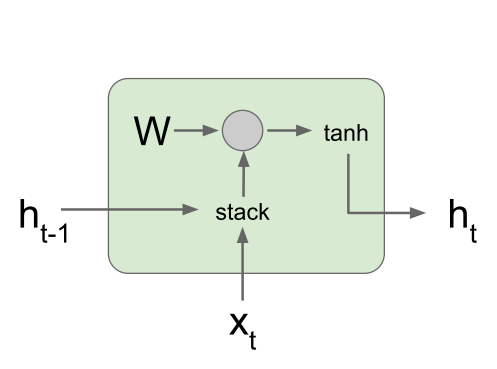
\includegraphics[width=.4\textwidth]{rnn.png}
	\caption{RNN unit}
\end{figure}

The forward pass of a RNN block can be mathematically described as:
\begin{equation}
h_t=f_W(h_{t-1},x_t)=W_h^T \cdot h_{t-1} + W_x^T \cdot x_t
\label{eqn:rnn}
\end{equation}

where $h_t$ is the current hidden state at time step $t$; $f_W$ the function -- either sigmoid or tanh -- that squashes the sum of the weight input and hidden state,  making gradients workable for backpropagation; $h_{t-1}$ the previous hidden state; $x_t$ the input at the same time step.

Recurrent networks rely on an extension of backpropagation called backpropagation through time, or BPTT. Time, in this case, is simply expressed by a well-defined, ordered series of calculations linking one time step to the next, which is all backpropagation needs to work.

However, RNNs suffer a lot from vanishing/exploding gradient problems. Intuitively, backpropagation from $h_t$ to $h_{t-1}$ multiplies by $W_h$, so computing gradient of $h_0$ involves many factors of $W_h$. If the largest singular value of $W_h$ is greater than $1$, then exploding gradients would occur; on the contrary if the largest singular value of $W_h$ if less than $1$, then vanishing gradients would happen. Exploding gradients can be solved relatively easily, because they can be truncated or squashed. Vanishing gradients can become too small for computers to work with or for networks to learn – a harder problem to solve. 

\paragraph{LSTM}
Long short-term memory was proposed to solve vanishing gradient problem of vanilla RNNs. LSTMs design complicated cells that help preserve the error that can be backpropagated through time and layers.

\begin{figure}[H]
	\centering
	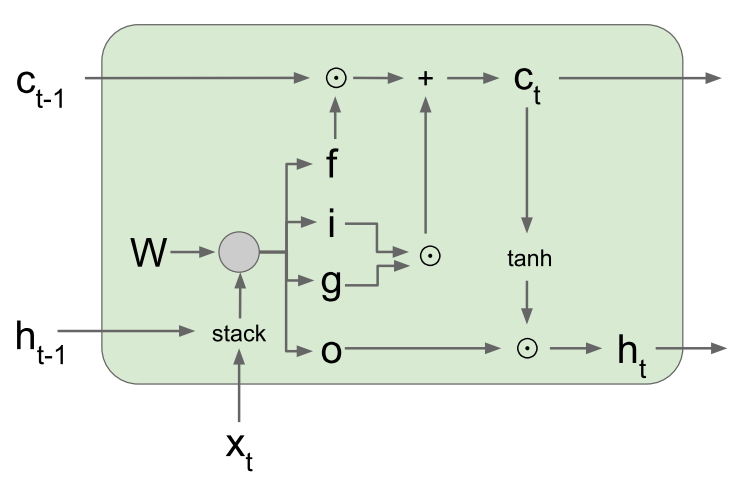
\includegraphics[width=.6\textwidth]{lstm.png}
	\caption{LSTM cell}
\end{figure}

The forward pass of a LSTM cell is defined as follows:
\begin{equation}
\begin{split}
\left(\begin{array}{c} i\\f\\o\\g \end{array}\right) &= \left(\begin{array}{c} \sigma\\\sigma\\\sigma\\\tanh \end{array}\right) W \left(\begin{array}{c} h_{t_1}\\x_t \end{array}\right)  \\  
c_t &= f \odot c_{t_1} + i \odot g\\
h_t &= o \odot \tanh(c_t)
\end{split}
\label{eqn:lstm}
\end{equation}
where $\odot$ is element-wise multiplication.

As described in equation\eqref{eqn:lstm}, all the computations involved, including sigmoid,  element-wise multiplication and so on, are differentiable, which are suitable for backpropagation. 

Those gates act on the signals they receive, and similar to the neural network’s nodes, they block or pass on information based on its strength and input, which they filter with their own sets of weights. Those weights, like the weights that modulate input and hidden states, are adjusted via the recurrent networks learning process. That is, the cells learn when to allow data to enter, leave or be deleted through the iterative process of making guesses, backpropagating error, and adjusting weights via gradient descent.

\subsection{Generative Models}
Neural network models we have learned so far, such as feed forward networks, CNNs, RNNs, LSTMs, are all basically discriminative models, which directly estimate posterior probabilities. Generative models focus on modeling class-conditional probabilistic distribution functions and prior probabilities, and a good outcome is that generative models can generate synthetic data points. Therefore generative adversarial networks become an active research field last year due to this feature. 

CS231 course discussed generative models like PixelRNN, PixelCNN, variational autoencoder and GAN, and used them to generate instances or do other interesting tasks. Although the theoretical derivations are difficult to understand, but perhaps the assignment will offer practical approach to better understanding.

\subsection{RNN - Implementation}
The forward pass of RNN is defined by equation\eqref{eqn:rnn}, and the code is simply one line:
\begin{lstlisting}
next_h = np.tanh(np.dot(x, Wx) + np.dot(prev_h, Wh) + b)
\end{lstlisting}

Since all the computations are differentiable, the backward pass is also simple:
\begin{lstlisting}
dh = (1 - next_h**2) * dnext_h
dx = np.dot(dh, Wx.T)
dprev_h = np.dot(dh, Wh.T)
dWx = np.dot(x.T, dh)
dWh = np.dot(prev_h.T, dh)
db = np.sum(dh, axis=0)
\end{lstlisting}

Above are what a RNN unit does in a single time step, but usually a RNN unit will process multiple time steps. At each iteration we should assign next\_h of last iteration to prev\_h of current iteration.

\subsection{LSTM - Implementation}
The implementation of LSTM uses a big matrix computed by weights W, hidden states h and input x, and then splits it to i, f, o, g gates.
\begin{lstlisting}
a = np.dot(x, Wx) + np.dot(prev_h, Wh) + b
ai, af, ao, ag = np.split(a, 4, axis=1)

i = sigmoid(ai)
f = sigmoid(af)
o = sigmoid(ao)
g = np.tanh(ag)

next_c = f * prev_c + i * g
next_h = o * np.tanh(next_c)
\end{lstlisting}

However, there is a tricky part in backward pass. Notice that $c_t$ also shows up in the equation that computes $h_t$, so $\nabla c_t$ backpropagated from next cell should also plus $\frac{\partial h_t}{\partial c_t}$.

\section{Plans}
In the next I plan to finish assignment 3 of cs231 and review generative model part of the course.

\end{document}
